\subsection{AST-Generation}
\label{chap:ast_generation}

Even though the CST already contains all relevant informations about the sources, it is very verbose and the structure of the CST is mostly not very friendly to work with.
Because of that, \verb|gp-modifiable-ast| implements modifiers purposed by \cite{GeneratingRewritableAST}, which are used to convert the CST into an AST.

The AST consists of three types of nodes. \verb|ProductionTreeNode| are nodes derived from a grammar production. 
\verb|TokenTreeNode| are nodes derived from a lexer token. 
\verb|StringTreeNode| are nodes that contain a string and are used to replace other tree nodes. 
The \verb|StringTreeNode| is not part of the initial AST. This node can be used by the user to replace subtrees in the finished AST or add a new node.
 
Any \verb|TokenTreeNode| which references a token from \verb|HIDDEN_LEXER_RULES| will marked as hidden. 
These nodes are stored in the AST, but are not visible to the user unless specifically requested. 
Next, the AST structure is modified by the modifiers defined in the grammar file. 
Each modifier has its own implementation and is applied bottom-up for each node.

\subsubsection{list-Modifier}

The \verb|list| modifier, intended by \cite{GeneratingRewritableAST}, is a modifier designed to flatten out self-recursive productions. This modifier can only be applied to symbols on the left side of a production. The following example could be a production for the function parameters in common programming languages.

\begin{lstlisting}[caption=list modifier example]
PARAMETER_LIST[list] -> PARAMETER_LIST PARAMETER | 
                        PARAMETER | 
                        EPSILON;
\end{lstlisting}

This grammar rule will generate the following CST for an input with three parameters.


\begin{figure}[H]
    \centering
    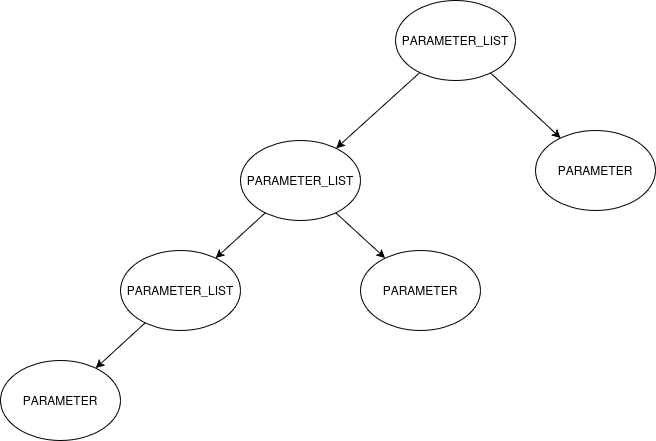
\includegraphics[scale=0.4]{"fig/list_modifier_cst.png"}
    \caption{CST before the list modifier is applied}
\end{figure}

This structure is too verbose and hard to work with in practice, by applying the \verb|[list]| modifier, we receive the following AST.

\begin{figure}[H]
    \centering
    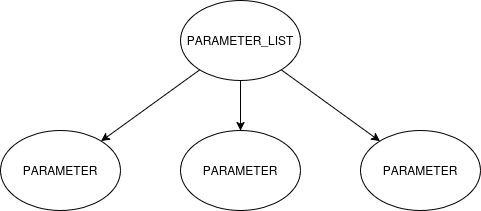
\includegraphics[scale=0.4]{"fig/list_modifier_ast.png"}
    \caption{AST after the list modifier is applied}
\end{figure}

This structure is much easier to manage and still contains all relevant informations about the sources.

The modifier is applied by checking if the children of the current \verb|ProductionTreeNode| $n$ contains a \verb|ProductionTreeNode| $m$ referencing the same production. If this is the case, $m$ is replaced in the children list of $n$ by all childrens of $m$.
As the modifiers are applied bottom-up this works for nested trees.

\subsubsection{alias-Modifier}

The \verb|alias| modifier, purposed by \cite{GeneratingRewritableAST}, is a modifier that can be applied to any symbol in the right hand side of a production. This modifier, will add an alias to the tree node, which can be used to search the tree. The following might be an example for a production for addition in a programming language.

\begin{verbatim}
ADD -> NUMBER[alias=left] plus NUMBER[alias=right];
\end{verbatim}

Without the alias modifier, the only way to differentiate between the both \verb|NUMBER| nodes would be by the order of the children of the \verb|ADD| tree node. The \verb|alias| modifier allows for cleaner searches in the AST.

This modifier is applied by simply storing the alias in the tree node.


\subsubsection{hidden-Modifier}

The \verb|hidden| modifier, purposed by \cite{GeneratingRewritableAST}, is a modifier that can be applied to terminal symbols in the right hand side of a production. This modifier will hide the tree node in the AST. In the previous example of the \verb|ADD| production, the \verb|ADD| tree node would have a \verb|TokenTreeNode| child, which references the \verb|plus| lexer definition. This information is obsolute, as the production will always contain this node and the production name already contains the necessary informations. By applying the \verb|hidden| modifier to the \verb|plus| symbol, the corresponding tree node will still be present, but not visible unless specifically requested.

\subsubsection{inline-Modifier}

The \verb|inline| modifier, purposed by \cite{GeneratingRewritableAST}, is a modifier that can be applied to nonterminal symbols in the right hand side of a production. 

By applying the modifier, the node will be replaced with all its children. This modifier should be used on nonterminals, which itself do not carry important informations, but their children do. This way all informations are maintaned, but the tree structure gets simplyfied.

\subsubsection{Not implemented modifiers}

\cite{GeneratingRewritableAST} purposed additional modifiers, those are not implemented currently. That would be the \verb|Boolean Access| modifier, which would replace a node with a boolean value. However, as we do not generate classes for each production, this would serve little purpose for us. The same reason applies to the \verb|superclass| modifier, which would create a hierarchy in the generated classes of the parser generator.
